\documentclass{article}
\usepackage{tikz}
\usepackage[margin=0.7in]{geometry}
\usepackage[utf8]{inputenc}

\title{CS 381 - A6}
\author{Martin Mueller}
\date{Due: April $10^{th}$, 2020}

\begin{document}
    \maketitle
    In order to construct a PDA $M$ that recognizes the language $A$ where $A = \{0, 1\}^{*} - \{0^{n}1^{n}$ $|$ $n \ge 0\}$, let us first consider what the language $A$ is. We know from the definition of $A$ that the compliment of $A$ contains exactly all the strings starting with some number of 0's and ending with that same number of 1's (including the empty string). Starting from here, we can now construct our rules and PDA for $A$ by accepting all strings that do no fit this rule. \\
    For a given input string $w = w_{0}, w_{1}...w_{n}$,
    \begin{enumerate}
        \item If $w$ is the empty string, stay at the start state, which does is not an accept state. We do this because the empty string is not in $A$.
        \item If $w_{0}$ is a 1, move into a perpetual accept state. All strings that start with 1 cannot start with 0.
        \item If $w$ starts with a 0, begin by pushing a dollar sign followed by a 0 on to the stack. This way, we can keep track of the number of 0's it reads.
        \item If $w$ contains only 0's, we stay in the accept state $q_{2}$ since $w$ has an unequal number of 1's and 0's.
        \item If $w$ contains 0's followed by 1's stay in an accept state until we encounter the dollar sign. If that happens, pop it and move to a non accept state. We do this because then we know $w$ is in the compliment of $A$.
        \item If we read an equal number of 0's and 1's followed by more input, move into a perpetual accept state since it would then be impossible for $w$ to be in the compliment of $A$.
    \end{enumerate}
    \begin{center}
        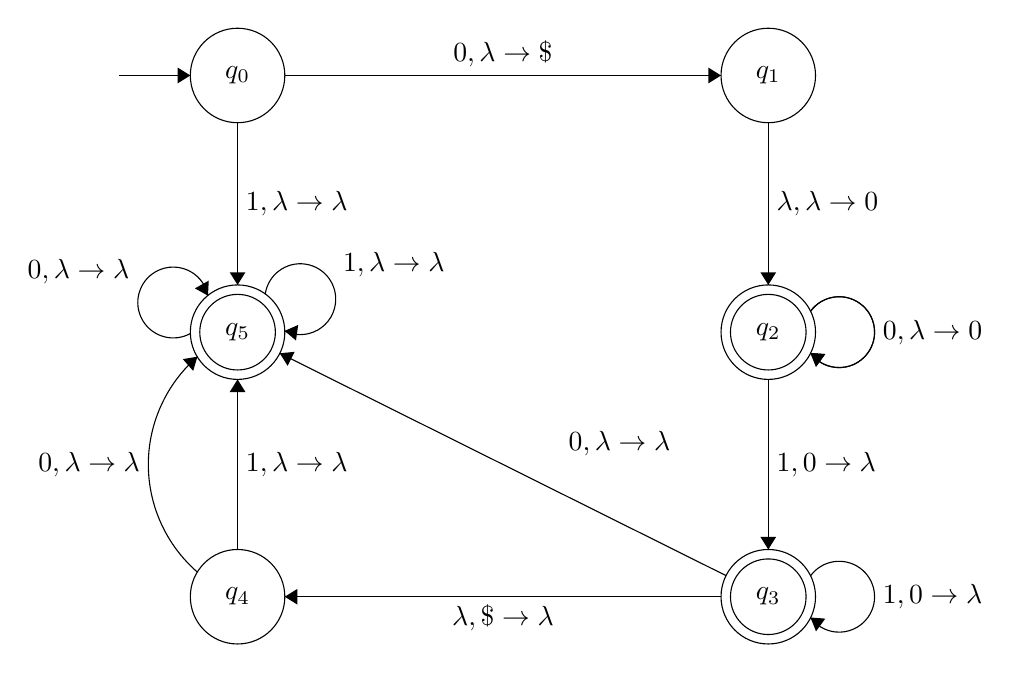
\begin{tikzpicture}[scale=0.2]
            \tikzstyle{every node}+=[inner sep=0pt]
            \draw [black] (57.4,-12.3) circle (3);
            \draw (57.4,-12.3) node {$q_1$};
            \draw [black] (57.4,-28.6) circle (3);
            \draw (57.4,-28.6) node {$q_2$};
            \draw [black] (57.4,-28.6) circle (2.4);
            \draw [black] (57.4,-45.4) circle (3);
            \draw (57.4,-45.4) node {$q_3$};
            \draw [black] (57.4,-45.4) circle (2.4);
            \draw [black] (23.7,-45.4) circle (3);
            \draw (23.7,-45.4) node {$q_4$};
            \draw [black] (23.7,-28.6) circle (3);
            \draw (23.7,-28.6) node {$q_5$};
            \draw [black] (23.7,-28.6) circle (2.4);
            \draw [black] (23.7,-12.3) circle (3);
            \draw (23.7,-12.3) node {$q_0$};
            \draw [black] (57.4,-15.3) -- (57.4,-25.6);
            \fill [black] (57.4,-25.6) -- (57.9,-24.8) -- (56.9,-24.8);
            \draw (57.9,-20.45) node [right] {$\lambda, \lambda \rightarrow 0$};
            \draw [black] (54.4,-45.4) -- (26.7,-45.4);
            \fill [black] (26.7,-45.4) -- (27.5,-45.9) -- (27.5,-44.9);
            \draw (40.55,-45.9) node [below] {$\lambda, \$ \rightarrow \lambda$};
            \draw [black] (57.4,-31.6) -- (57.4,-42.4);
            \fill [black] (57.4,-42.4) -- (57.9,-41.6) -- (56.9,-41.6);
            \draw (57.9,-37) node [right] {$1, 0 \rightarrow \lambda$};
            \draw [black] (60.08,-27.277) arc (144:-144:2.25);
            \fill [black] (60.08,-29.92) -- (60.43,-30.8) -- (61.02,-29.99);
            \draw [black] (60.08,-27.277) arc (144:-144:2.25);
            \draw (64.65,-28.6) node [right] {$0, \lambda \rightarrow 0$};
            \fill [black] (60.08,-29.92) -- (60.43,-30.8) -- (61.02,-29.99);
            \draw [black] (60.08,-44.077) arc (144:-144:2.25);
            \draw (64.65,-45.4) node [right] {$1, 0 \rightarrow \lambda$};
            \fill [black] (60.08,-46.72) -- (60.43,-47.6) -- (61.02,-46.79);
            \draw [black] (25.456,-26.182) arc (171.73593:-116.26407:2.25);
            \draw (30.36,-24.31) node [right] {$1, \lambda \rightarrow \lambda$};
            \fill [black] (26.69,-28.52) -- (27.41,-29.13) -- (27.55,-28.14);
            \draw [black] (20.713,-28.679) arc (299.24083:11.24083:2.25);
            \draw (16.85,-24.74) node [left] {$0, \lambda \rightarrow \lambda$};
            \fill [black] (21.82,-26.28) -- (21.87,-25.33) -- (20.99,-25.82);
            \draw [black] (26.7,-12.3) -- (54.4,-12.3);
            \fill [black] (54.4,-12.3) -- (53.6,-11.8) -- (53.6,-12.8);
            \draw (40.55,-11.8) node [above] {$0, \lambda \rightarrow \$$};
            \draw [black] (23.7,-15.3) -- (23.7,-25.6);
            \fill [black] (23.7,-25.6) -- (24.2,-24.8) -- (23.2,-24.8);
            \draw (24.2,-20.45) node [right] {$1, \lambda \rightarrow \lambda$};
            \draw [black] (23.7,-42.4) -- (23.7,-31.6);
            \fill [black] (23.7,-31.6) -- (23.2,-32.4) -- (24.2,-32.4);
            \draw (24.2,-37) node [right] {$1, \lambda \rightarrow \lambda$};
            \draw [black] (21.153,-43.841) arc (-130.96333:-229.03667:9.059);
            \fill [black] (21.15,-30.16) -- (20.22,-30.31) -- (20.88,-31.06);
            \draw (17.53,-37) node [left] {$0, \lambda \rightarrow \lambda$};
            \draw [black] (54.72,-44.06) -- (26.38,-29.94);
            \fill [black] (26.38,-29.94) -- (26.88,-30.74) -- (27.32,-29.85);
            \draw (47.95,-36.46) node [above] {$0, \lambda \rightarrow \lambda$};
            \draw [black] (16.2,-12.3) -- (20.7,-12.3);
            \fill [black] (20.7,-12.3) -- (19.9,-11.8) -- (19.9,-12.8);
        \end{tikzpicture}
    \end{center}
\end{document}
